\documentclass[aspectratio=169]{beamer}

% Pacotes
\usepackage{lipsum}
\usepackage{caption}
\usepackage{graphicx}
    \DeclareCaptionFormat{sanslabel}{#3}%
\usepackage{color}
\usepackage[table]{xcolor}
\usepackage{tikz}
\usepackage{tcolorbox}
\usepackage{amsmath}
\usepackage{amsfonts}
\usepackage{amssymb}
\usepackage{mathrsfs}
\usepackage{mathtools}
\usepackage{enumitem} 
\usepackage{float}
\usepackage[utf8]{inputenc}	
\usepackage[french]{babel}
\usepackage[T1]{fontenc}
\usepackage{caption}
\usepackage{subcaption}


% Theme choice:
\usetheme{CambridgeUS}

% Cores personalizadas
\definecolor{PROFMATgreen}{RGB}{0, 138, 163}
\definecolor{UFTgreen}{RGB}{0, 137, 124}
\definecolor{UFTblue}{RGB}{0, 84, 132}
\definecolor{UFTyellow}{RGB}{253, 185, 46}
\definecolor{UFTgray}{RGB}{132, 134, 136}

% Ativar numeração de tabelas
\setbeamertemplate{caption}[numbered]

% Definir novo estilo de item com quadrado verde
\setlist[itemize,1]{label=\textcolor{UFTgreen}{\rule{1ex}{1ex}}}

\setbeamercolor*{structure}{bg=UFTgreen,fg=black}

\setbeamercolor*{palette primary}{fg=black,bg=PROFMATgreen}
\setbeamercolor*{palette secondary}{fg=white,bg=UFTblue}
\setbeamercolor*{palette tertiary}{fg=black,bg=UFTgreen}
\setbeamercolor*{palette quaternary}{fg=white,bg=black}

\setbeamercolor{section in toc}{fg=black,bg=white}
\setbeamercolor{alerted text}{fg=white}

\setbeamercolor*{item}{fg=PROFMATgreen}

\setbeamercolor{block title}{bg=UFTgreen,fg=white}
\setbeamercolor{block body}{bg=UFTgray!10,fg=black}

\setbeamercolor{titlelike}{fg=white, bg=UFTblue}
\setbeamercolor{frametitle}{bg=UFTgray!20,fg=UFTgreen}


\setbeamertemplate{title page}{
    \vfill
    \vskip1em\par
    \begingroup
        \centering
        \begin{beamercolorbox}[sep=8pt,center,shadow=true,rounded=false]{title}
            \usebeamerfont{title}\inserttitle\par%
            \ifx\insertsubtitle\@empty%
            \else%
                \vskip0.25em%
                {\usebeamerfont{subtitle}\usebeamercolor[fg]{subtitle}\insertsubtitle\par}%
            \fi%
        \end{beamercolorbox}%
        \vskip0.5em\par
        \begin{minipage}{0.6\linewidth}
            \centering
            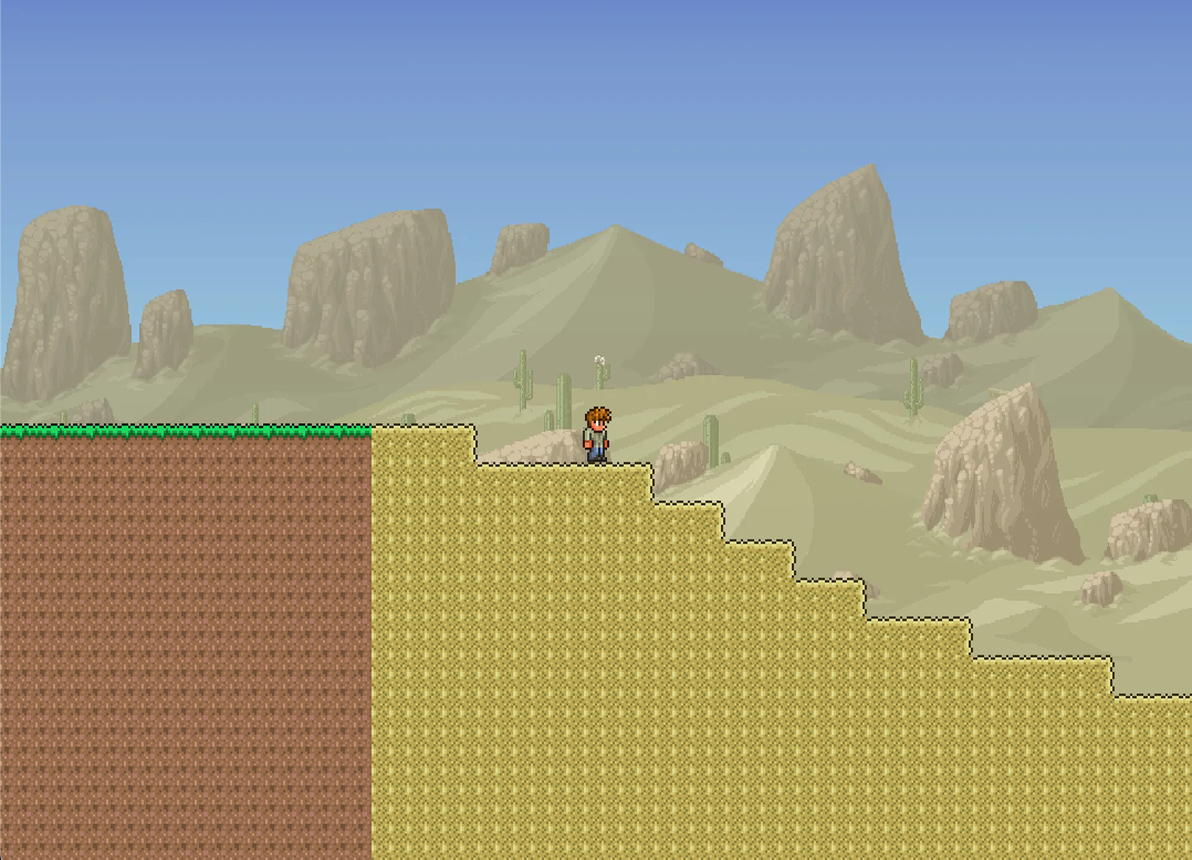
\includegraphics[width=0.6\linewidth]{assets/background_1.png}
        \end{minipage}
        \begin{beamercolorbox}[sep=6pt,center]{author}
            \usebeamerfont{author}\insertauthor
        \end{beamercolorbox}
        \begin{beamercolorbox}[sep=5pt,center]{advisor}
            \usebeamerfont{institute} \advisorname
        \end{beamercolorbox}
        \begin{beamercolorbox}[sep=5pt,center]{institute}
            \usebeamerfont{institute}\insertinstitute
        \end{beamercolorbox}
        \par
    \endgroup
    \vfill
}


% Remover bordas arredondadas dos blocks
\makeatletter
\setbeamertemplate{blocks}[default] % Isso remove o arredondamento
\makeatother


% Pacotes de citações
% ---

\usepackage[alf,abnt-etal-text=it,abnt-repeated-author-omit=yes,abnt-etal-list=0,abnt-etal-cite=3,abnt-emphasize=bf]{abntex2cite}	% Citações padrão ABNT



\setbeamercolor{bibliography entry author}{fg=black}
\setbeamertemplate{bibliography item}{\newblock}


\setbeamertemplate{frametitle continuation}{}

% Redefinir o separador para um traço
% Redefinir o separador
\captionsetup[figure]{labelformat=simple, labelsep=endash, textformat=period, font=footnotesize}


% Redefine espaçamento antes e depois da legenda em figuras e tabelas
\captionsetup[figure]{aboveskip=2pt, belowskip=0pt}


% Define uma penalidade alta para a hifenização
\hyphenpenalty=10000
\tolerance=10000


% Personalizando o estilo da tabela de conteúdos
\setbeamertemplate{section in toc}[sections numbered]
\renewcommand{\thesection}{\textcolor{PROFMATgreen}{\arabic{section}}}
\renewcommand{\thesubsection}{\textcolor{PROFMATgreen}{\arabic{section}.\arabic{subsection}}}

\setbeamersize{text margin left=0.8cm, text margin right=0.8cm}



% Informações do documento
\title[Génération procédurale]{Génération procédurale de décors}
\subtitle{Projet de recherche documentaire}
\author[K.Mathias, M.Girardclos]{Killian Mathias et Matthéo Girardclos}
\institute[UMLP]{Université Marie et Louis Pasteur}
\date{2024 - 2025}

% Definir o nome do orientador
\newcommand{\advisorname}{\textbf{Superviseur :} M. Pierre-Cyrille Héam}




\begin{document}

\begin{frame}
    \titlepage
\end{frame}

\begin{frame}[t]{Sommaire}
    \tableofcontents[hideallsubsections]
\end{frame}


\section{Introduction}

\begin{frame}{Introduction}
    La génération procédurale en informatique permet de créer automatiquement du contenu numérique varié, notamment dans les jeux vidéo, en s’appuyant sur des algorithmes. Ce projet vise à développer une version simplifiée de Terraria, en mettant l’accent sur la génération du monde, des biomes et des grottes.
    \vfill
    \begin{figure}[!h]
        \centering
        \begin{subfigure}[b]{0.3\textwidth}
            \centering
            
\includegraphics[width=0.5\textwidth]{assets/nomanssky.png}
        \end{subfigure}
        \hspace{-1cm}
        \begin{subfigure}[b]{0.3\textwidth}
            \centering
            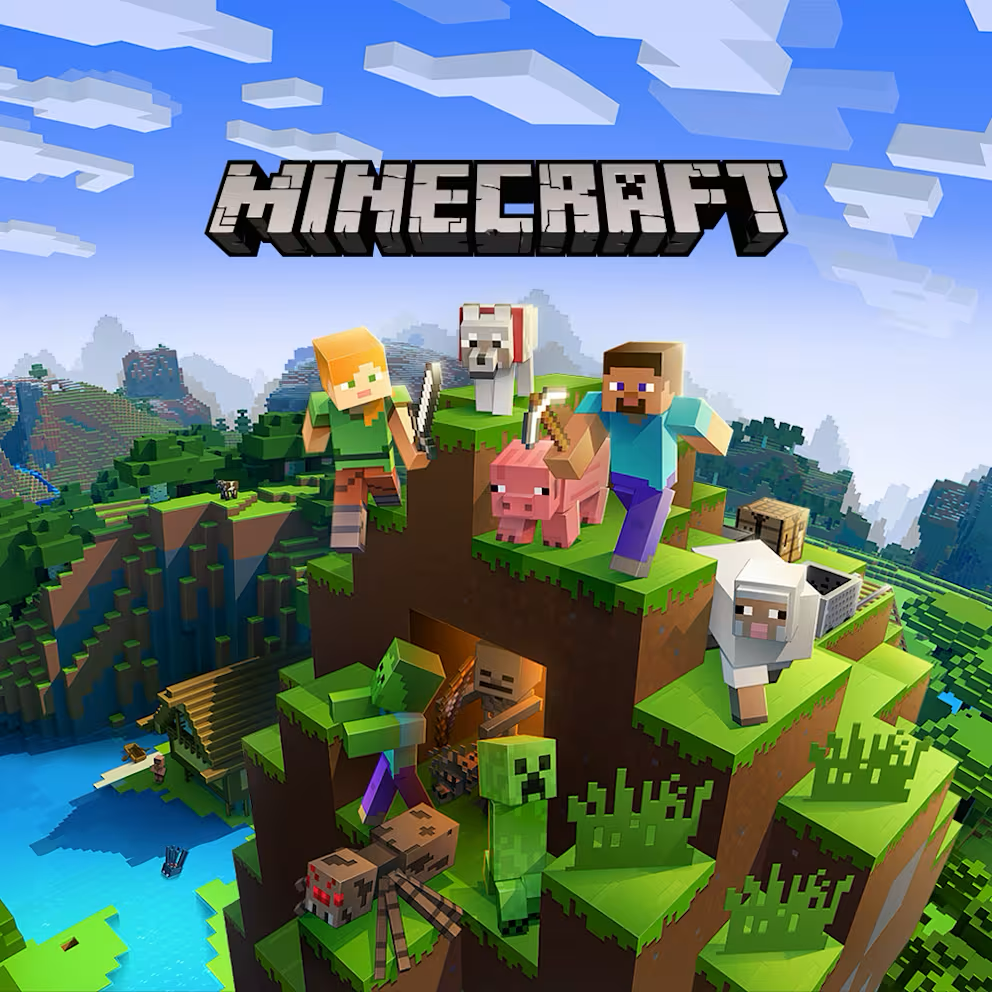
\includegraphics[width=0.5\textwidth]{assets/minecraft.png}
        \end{subfigure}
    \end{figure}
\end{frame}


\section{Technologies et approches}

\begin{frame}{Technologies et approches}
    \tableofcontents[sections={2}]
\end{frame}

\subsection{Génération de terrains et de reliefs}

\begin{frame}{Génération de terrains et de reliefs}
    \begin{columns}
        \centering
        \begin{column}{0.5\textwidth}
            \centering
            \begin{itemize}
                \item Deux algorithmes utilisés : \textbf{bruit de Perlin} et \textbf{bruit Simplex}.
                \item \textbf{Bruit de Perlin} (1985) : Ken Perlin, pseudo-aléatoire, 2D/3D, décors procéduraux.
                \item \textbf{Bruit Simplex} (2001) : Ken Perlin, optimisation, > 3D, plus rapide, moins documenté.
            \end{itemize}
        \end{column}
        \begin{column}{0.5\textwidth}
            \centering
            \begin{figure}
                \centering
                \captionsetup{format=sanslabel}
                
\includegraphics[width=0.5\textwidth]{assets/Perlin_noise.jpg}
                \caption{Bruit de Perlin à 2 dimensions}
            \end{figure}
        \end{column}
    \end{columns}
\end{frame}

\subsection{Génération de biomes}

\begin{frame}{Génération de biomes}
    \begin{columns}
        \centering
        \begin{column}{0.5\textwidth}
            \centering
            \begin{itemize}
                \item \textbf{Biomes} : zones, textures, caractéristiques
                \item \textbf{Méthodes} : bruit Worley, carte température/humidité
                \item \textbf{Bruit Worley} : Voronoï, transitions brusques, peu adapté
                \item \textbf{Température/humidité} : Perlin, transitions douces, réutilisation algorithme
                \item \textbf{Choix} : approche température/humidité
            \end{itemize}
        \end{column}
        \begin{column}{0.5\textwidth}
            \centering
            \begin{figure}
                \centering
                \captionsetup{format=sanslabel}
                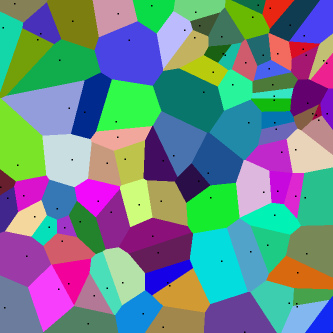
\includegraphics[width=0.3\textwidth]{assets/voronoi.png}
                \caption{Diagramme de Voronoï}
            \end{figure}
            \begin{figure}
                \centering
                \captionsetup{format=sanslabel}
                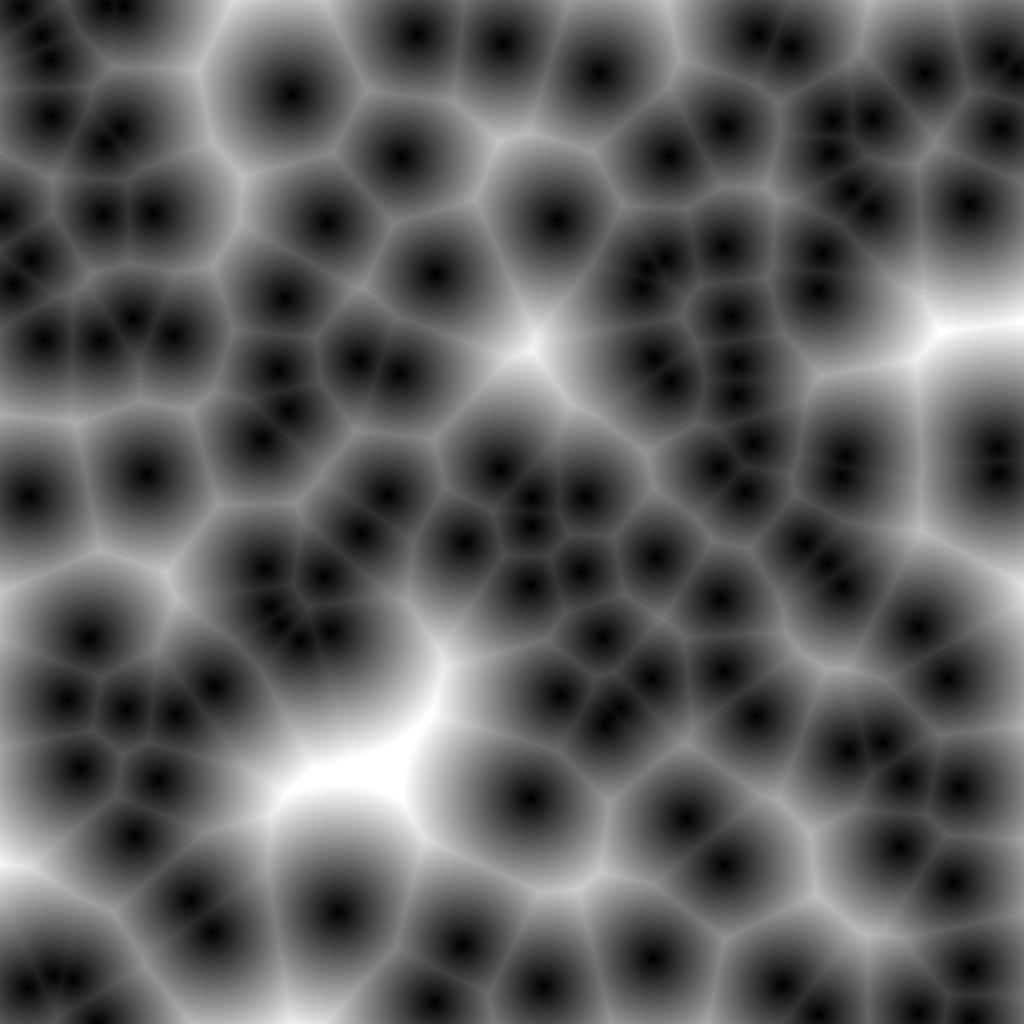
\includegraphics[width=0.3\textwidth]{assets/Worley.jpg}
                \caption{Bruit de Worley}
            \end{figure}
        \end{column}
    \end{columns}
\end{frame}

\subsection{Génération de grottes et de cavernes}

\begin{frame}{Génération de grottes et de cavernes}
    \begin{columns}
        \centering
        \begin{column}{0.5\textwidth}
            \centering
            \begin{itemize}
                \item \textbf{Méthodes} : Random Walk, automates cellulaires
                \item \textbf{Random Walk} : donjons, tunnels, éloigné de Terraria
                \item \textbf{Automates cellulaires} : grille, évolution cellules, grottes réalistes, utilisé par Terraria
            \end{itemize}
        \end{column}
        \begin{column}{0.5\textwidth}
            \centering
            \begin{figure}
                \centering
                \captionsetup{format=sanslabel}
                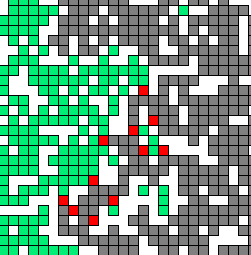
\includegraphics[width=0.5\textwidth]{assets/automate_cellulaire.png}
                \caption{Automate cellulaire}
            \end{figure}
        \end{column}
    \end{columns}
\end{frame}

\subsection{Génération de minerais et ressources}

\begin{frame}{Génération de minerais et ressources}
    \begin{columns}
        \centering
        \begin{column}{0.5\textwidth}
            \centering
            \begin{itemize}
                \item \textbf{Méthodes} : stratification, Perlin appliqué aux minerais
                \item \textbf{Stratification} : couches, utilisé par Minecraft, combiné avec Perlin
                \item \textbf{Perlin} : intégré au terrain, utilisé par Terraria
            \end{itemize}
        \end{column}
        \begin{column}{0.5\textwidth}
            \centering
            \begin{figure}
                \centering
                \captionsetup{format=sanslabel}
                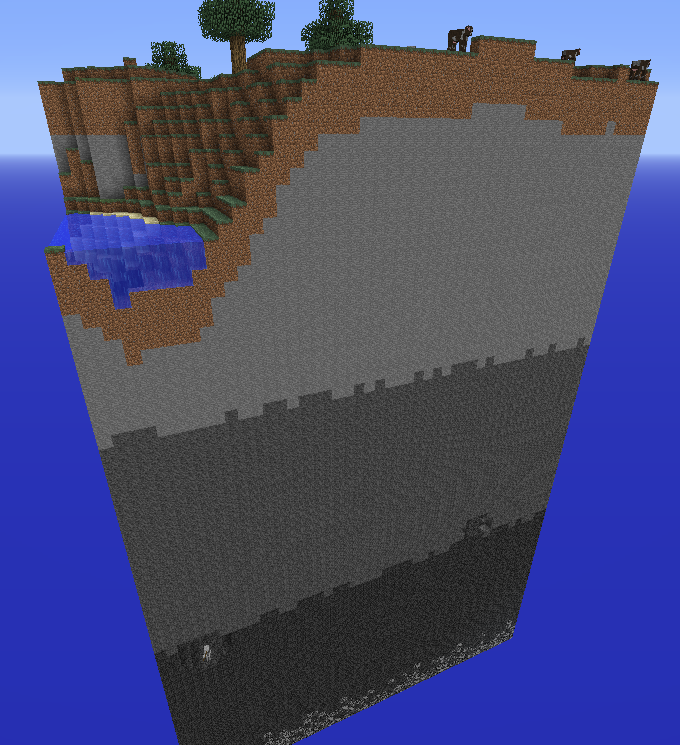
\includegraphics[width=0.5\textwidth]{assets/stratification.png}
                \caption{Distribution par couches de Minecraft}
            \end{figure}
        \end{column}
    \end{columns}
\end{frame}


\section{Méthodologie}

\begin{frame}{Méthodologie}
    \tableofcontents[sections={3}]
\end{frame}

\subsection{Outils utilisés}

\begin{frame}{Outils utilisés}
    \centering
    \begin{tikzpicture}[scale=1, every node/.style={anchor=center}]
        \node at (3, 6) {
\includegraphics[width=2.3cm]{assets/python_logo.png}};
        \node at (9, 6) {
\includegraphics[width=2.8cm]{assets/pygame_logo.png}};

        \node at (1.5, 2.5) {
\includegraphics[width=2.3cm]{assets/discord.png}};
        \node at (6, 2.5) {
\includegraphics[width=2.5cm]{assets/git.png}};
        \node at (10.5, 2.5) {
\includegraphics[width=2.5cm]{assets/jira.png}};
    \end{tikzpicture}
\end{frame}

\subsection{Analyse du jeu}

\begin{frame}{Analyse du jeu}
    \begin{columns}
        \centering
        \begin{column}{0.5\textwidth}
            \centering
            \begin{itemize}
                \item \textbf{Terraria} : bac à sable, aventure, construction, Re-Logic, 2011
                \item \textbf{Gameplay} : monde procédural, outils, inventaire, blocs, crafting
                \item \textbf{Carte} : 2D verticale, montagnes, lacs, forêts, biomes, souterrains
                \item \textbf{Souterrain} : minerais, grottes, architectures, creusage
                \item \textbf{Objectif projet} : génération terrain, altitude, biomes, sous-sols (minerais, cavernes)
            \end{itemize}
        \end{column}
        \begin{column}{0.5\textwidth}
            \centering
            \begin{figure}
                \centering
                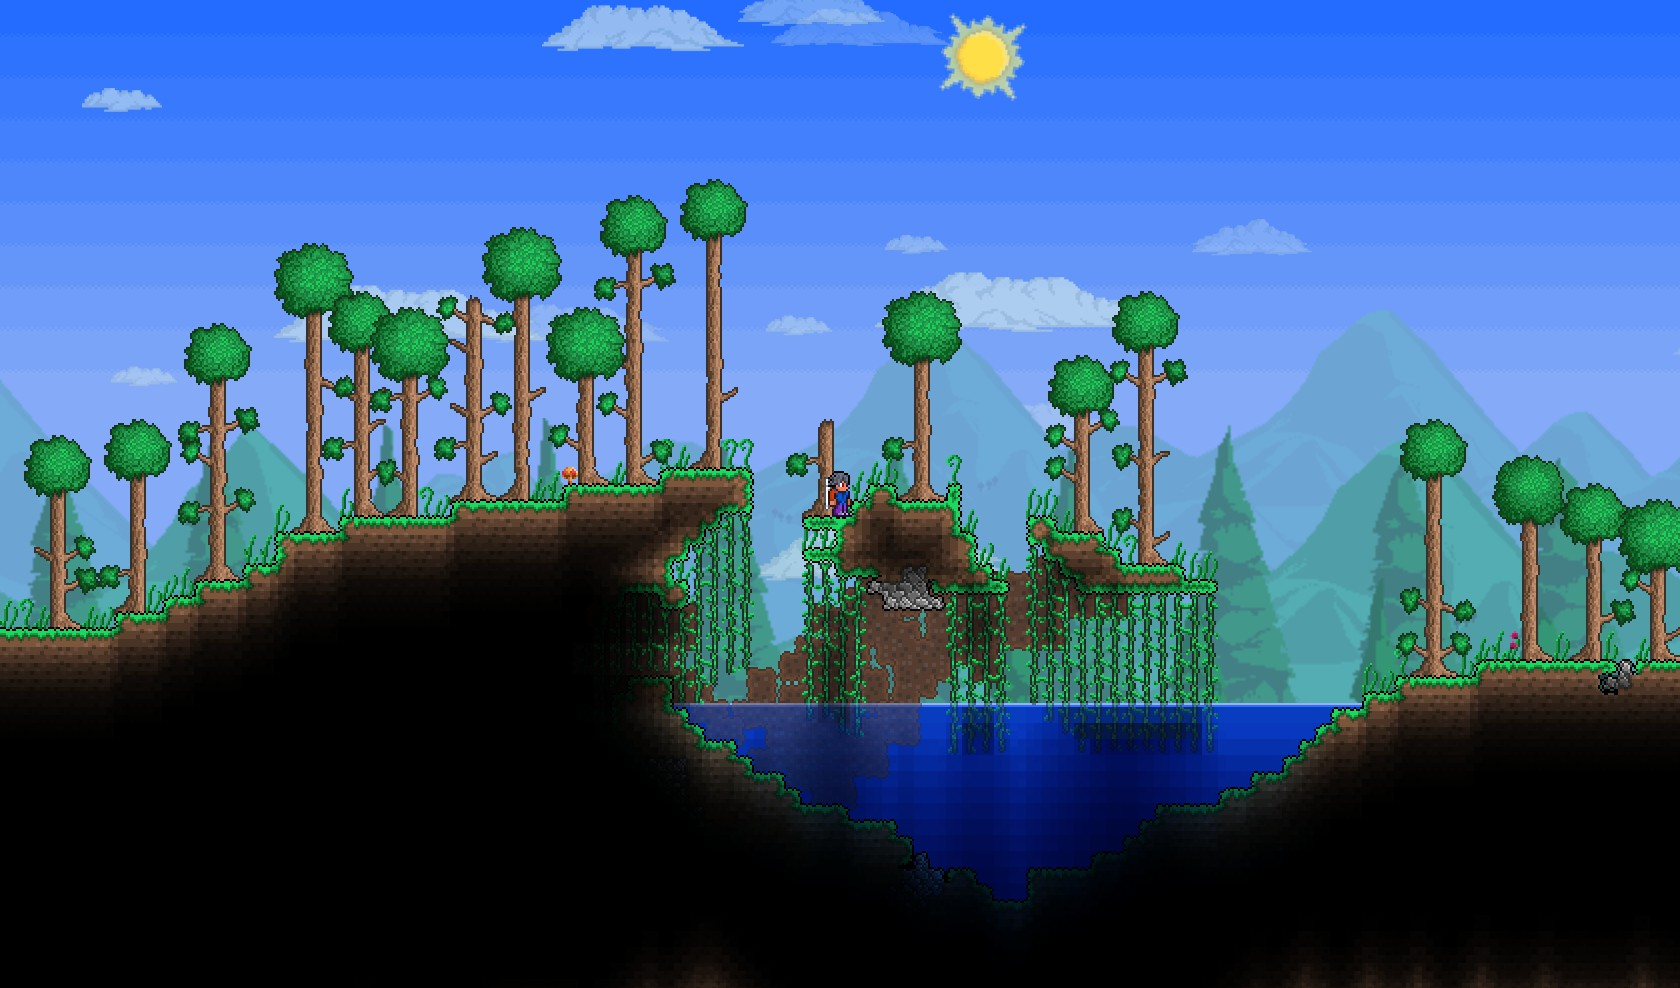
\includegraphics[width=0.7\textwidth]{assets/terraria_forest_biome.jpg}
            \end{figure}
            \begin{figure}
                \centering
                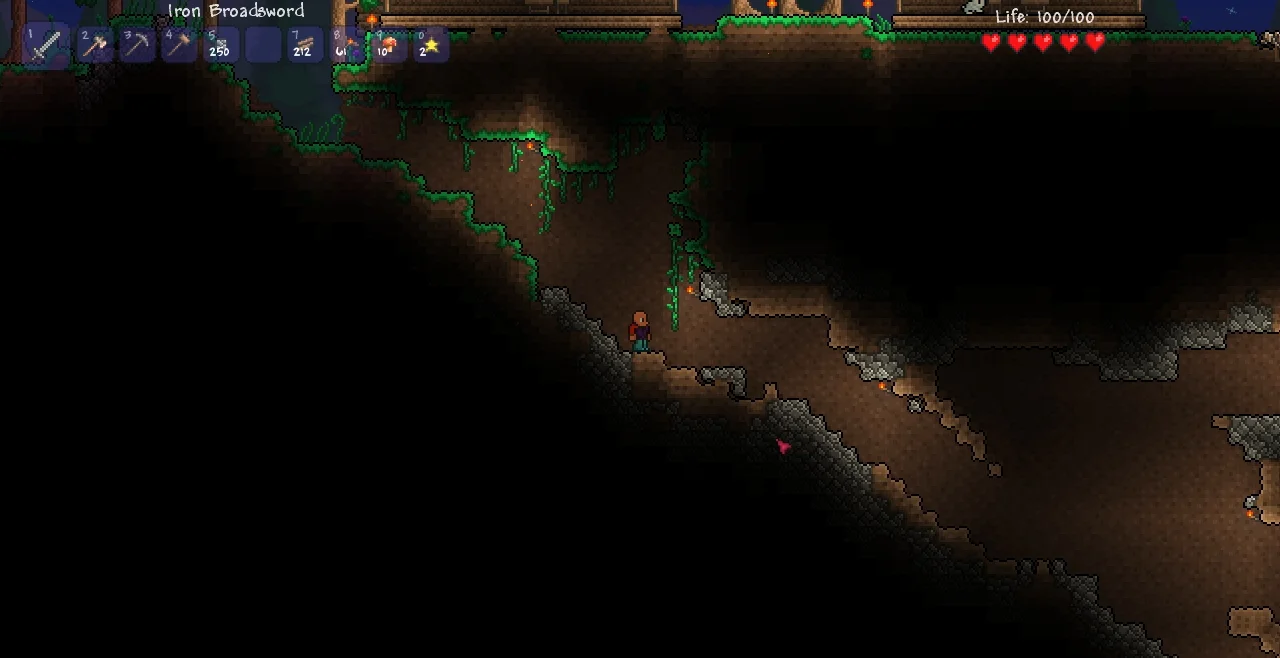
\includegraphics[width=0.7\textwidth]{assets/terraria_cavern.png}
            \end{figure}
        \end{column}
    \end{columns}
\end{frame}

\subsection{Organisation du code}

\begin{frame}{Organisation du code}
    \begin{figure}
        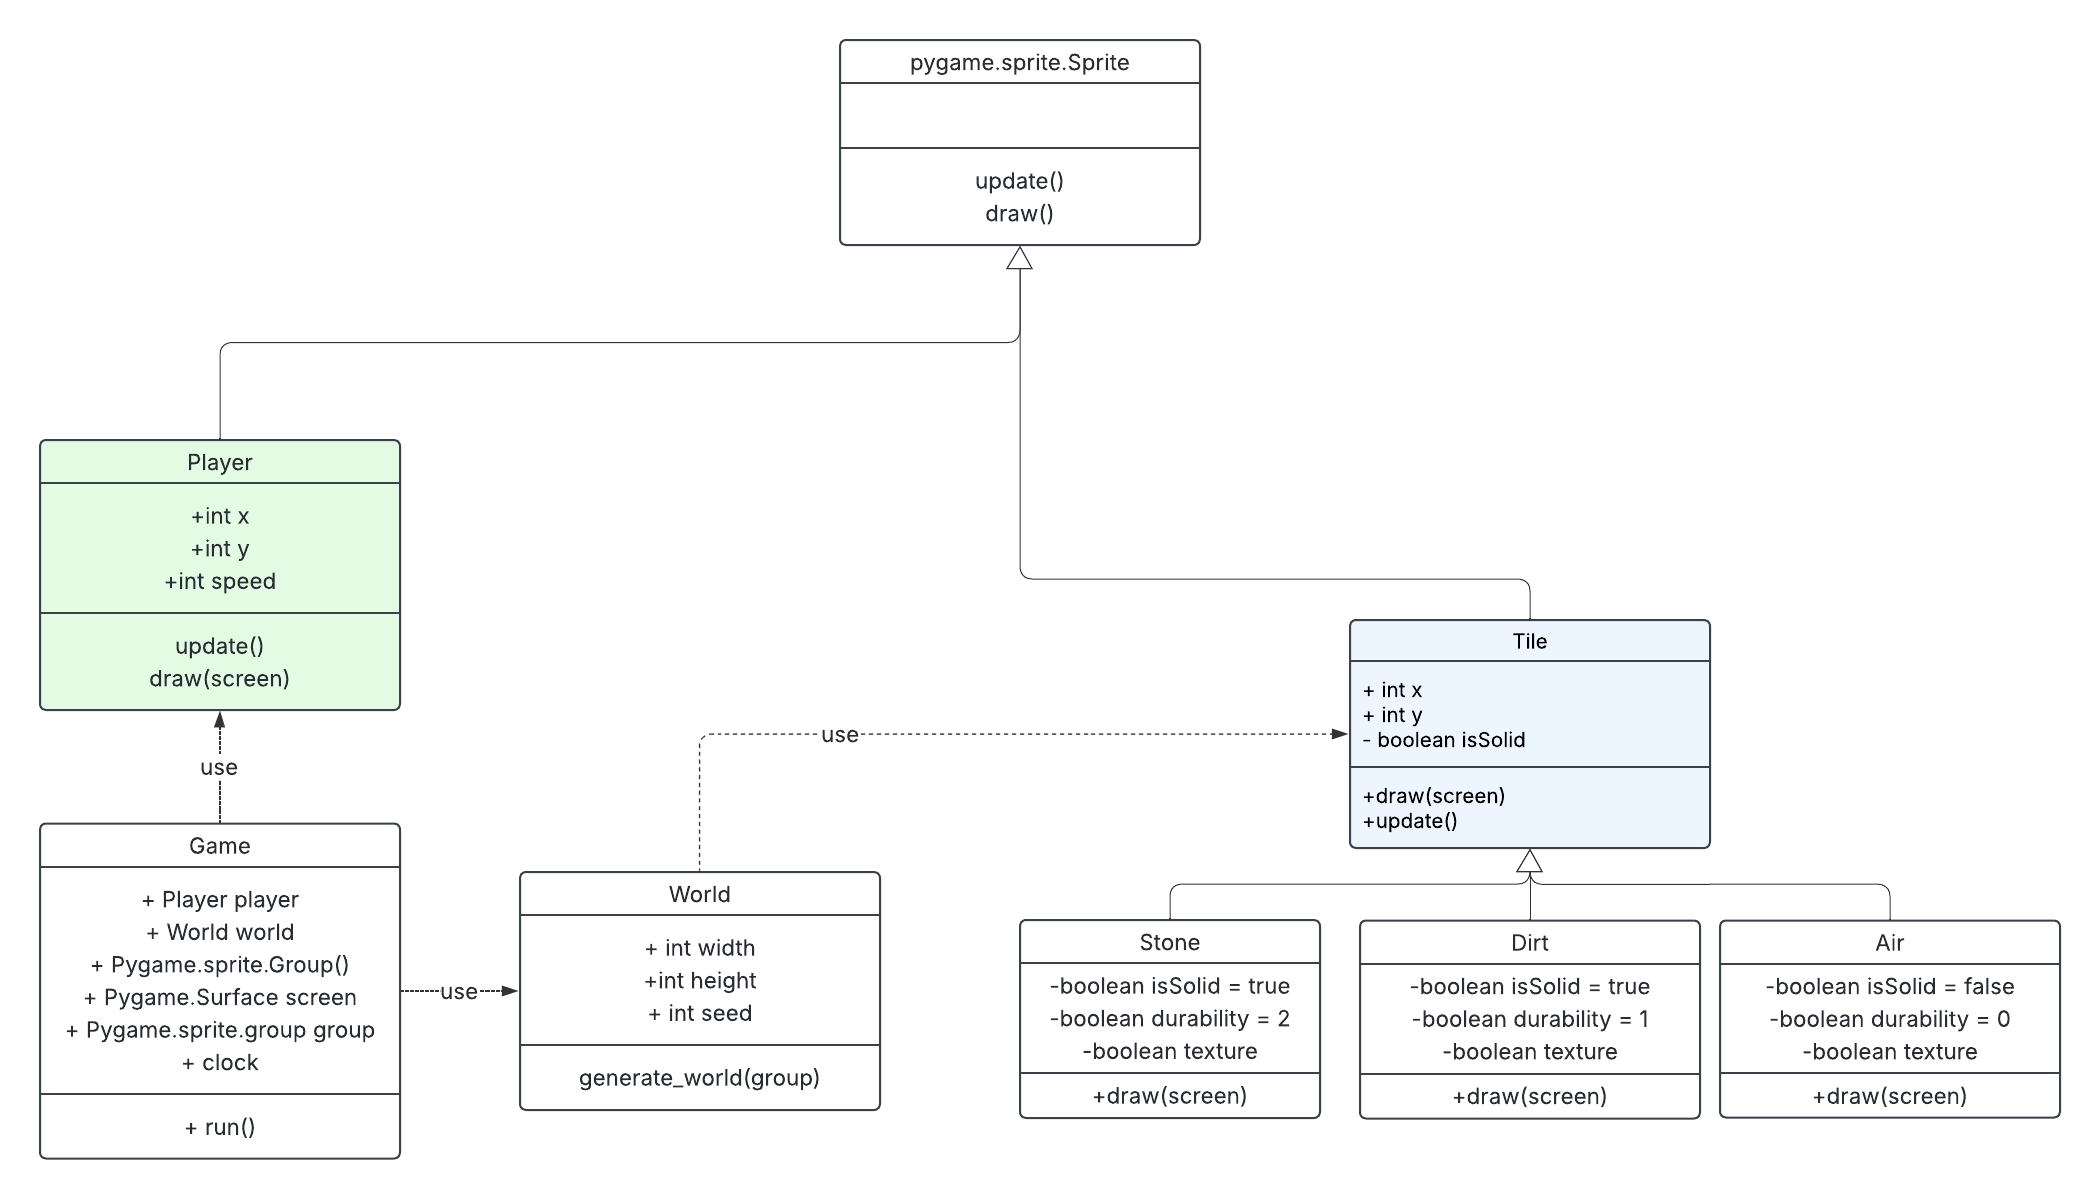
\includegraphics[height=0.8\textheight]{assets/UML_class.png}
    \end{figure}
\end{frame}


\section{Implémentation}

\begin{frame}{Implémentation}
    \tableofcontents[sections={4}]
\end{frame}

\subsection{Bases du jeu}

\begin{frame}{Bases du jeu}
    \centering
    \begin{itemize}
        \item \textbf{Fenêtre de jeu} avec Pygame
        \item \textbf{Boucle de jeu principale}(Gestion des événements)
        \item \textbf{Joueur} : \\
        - Boîte de collision\\
        - Déplacement (horizontal, saut et gravité)\\
        - Animation
        
    \end{itemize}
\end{frame}

\subsection{Génération procédurale du terrain}

\begin{frame}{Génération procédurale du terrain}
    \begin{columns}
        \centering
        \begin{column}{0.5\textwidth}
            \centering
            \begin{itemize}
                \item \textbf{Choix technique} : bruit de Perlin 1 dimension, algorithme léger
                \item \textbf{Processus} :\\
                    - Tableau valeurs aléatoires (-1 à 1)\\
                    - Lissage 100 fois avec Perlin\\
                    - Valeurs multipliées par hauteur max\\
                    - Transitions douces
                \item \textbf{Résultat} : terrain avec relief réaliste
                \item \textbf{Blocs} : herbe en haut, terre dessous, air ailleurs\\
            \end{itemize}
        \end{column}
        \begin{column}{0.5\textwidth}
            \centering
            \begin{figure}
                \centering
                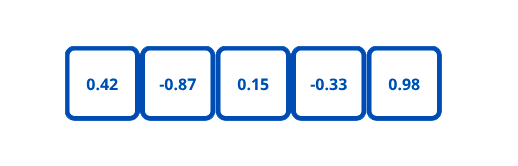
\includegraphics[width=0.9\textwidth]{assets/tableau.png}
            \end{figure}
            \begin{figure}
                \centering
                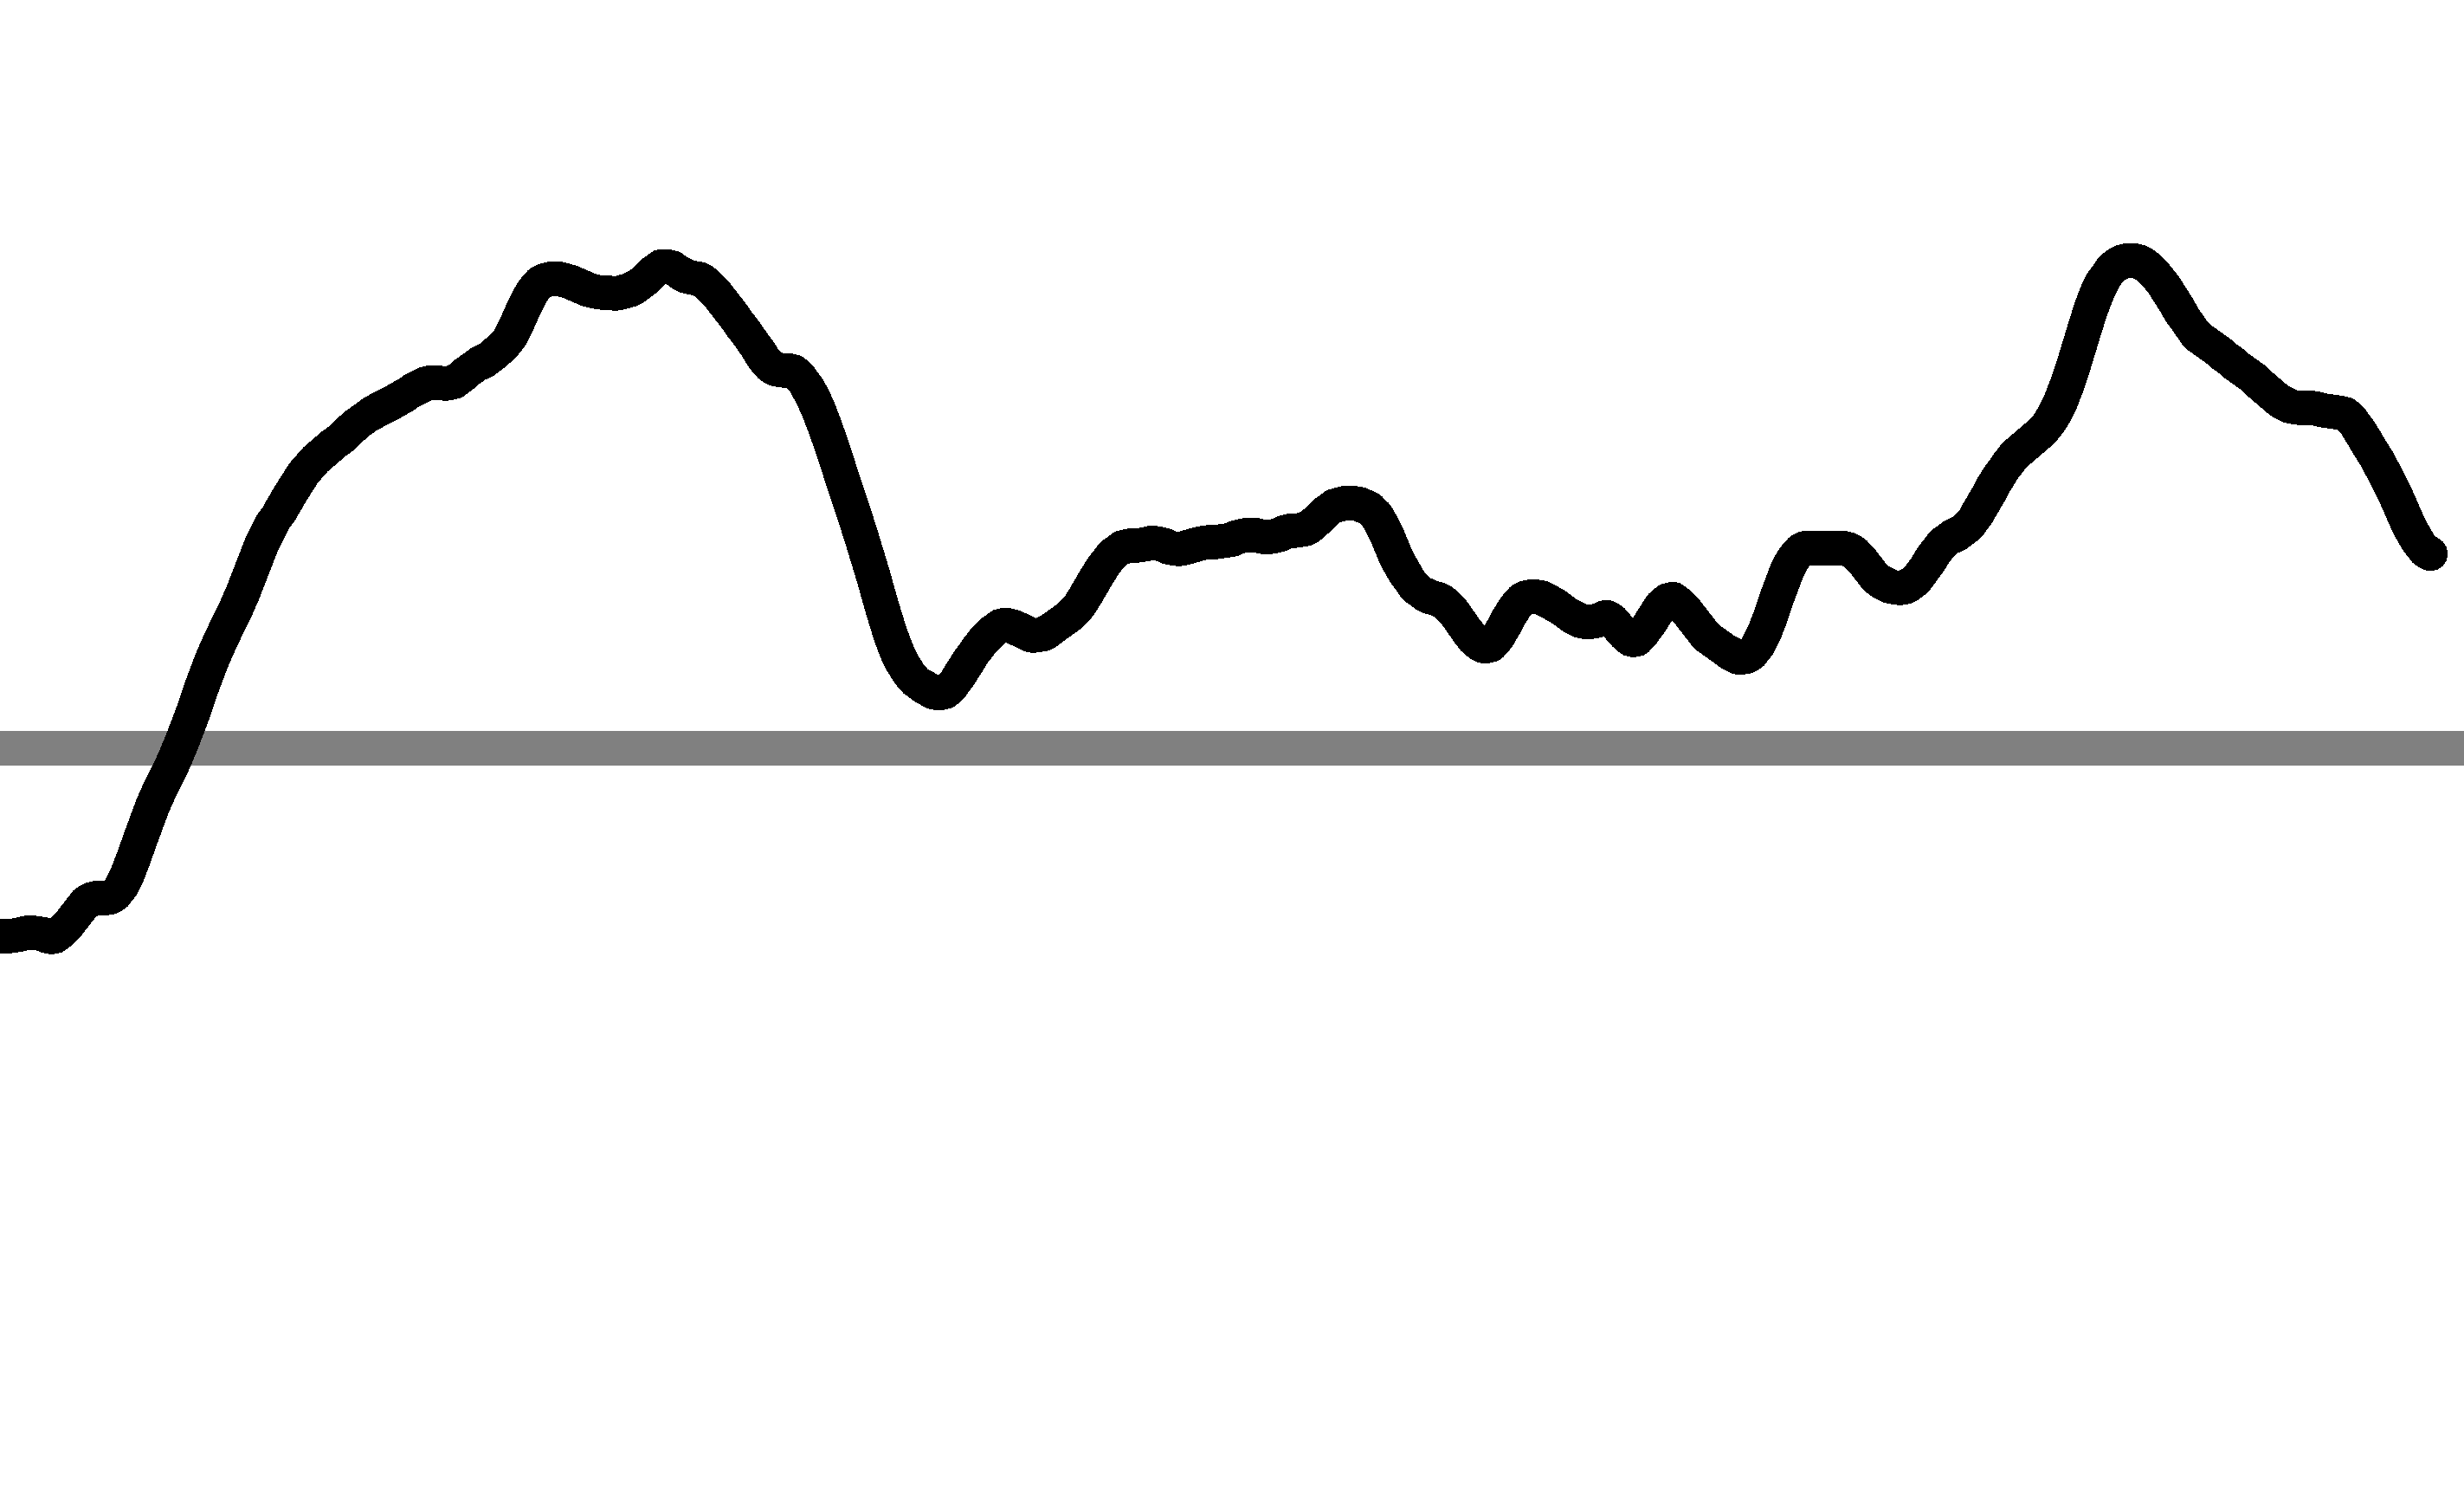
\includegraphics[width=0.7\textwidth]{assets/PerlinNoise1d.png}
            \end{figure}
        \end{column}
    \end{columns}
\end{frame}

\subsection{Collisions et fonctionnalité}

\begin{frame}{Collisions et fonctionnalité}
    \begin{columns}
        \centering
        \begin{column}{0.5\textwidth}
            \centering
            \begin{itemize}
                \item \textbf{Joueur et tuiles} avec rect Pygame\\
                \item collide\_rect pour détecter collisions
                \item \textbf{Empêcher déplacement} si collision\\
                
            \end{itemize}
            % \begin{itemize}
            %     \item \textbf{Terrain} : fonctionnel, collisions absentes
            %     \item \textbf{Joueur et tuiles avec rect Pygame}
            %     \item collide_rect pour détecter collisions
            %     \item \textbf{Blocs} : herbe en haut, terre dessous, air ailleurs\\
            % \end{itemize}
        \end{column}
        \begin{column}{0.5\textwidth}
            \centering
            \begin{figure}
                \centering
                \captionsetup{format=sanslabel}
                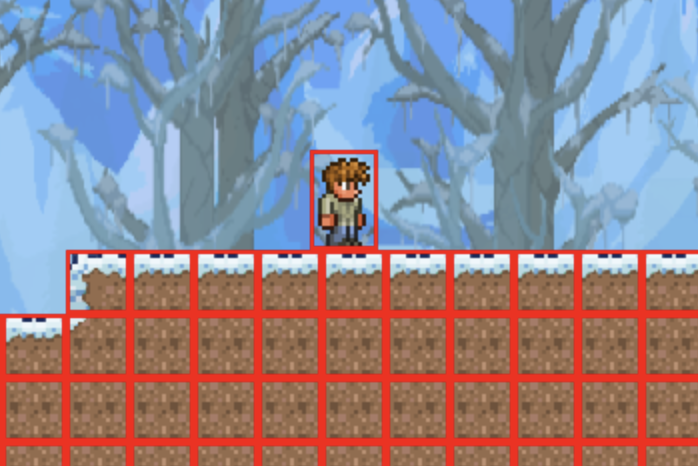
\includegraphics[width=0.5\textwidth]{assets/hit_box.png}
            \end{figure}
            \begin{figure}
                \centering
                \captionsetup{format=sanslabel}
                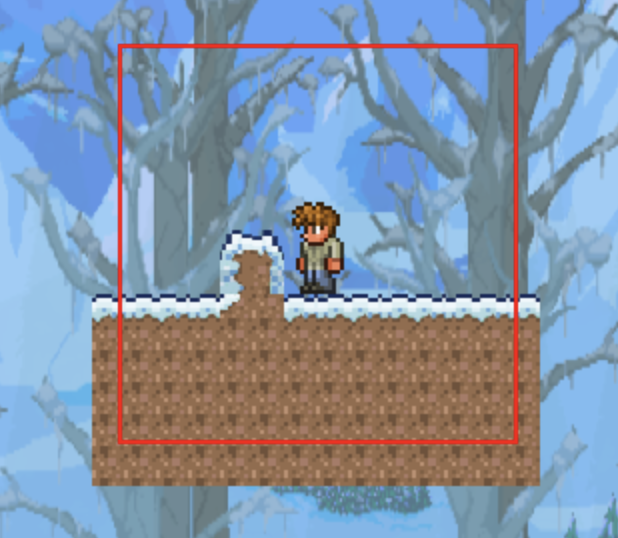
\includegraphics[width=0.5\textwidth]{assets/camera.png}
            \end{figure}
        \end{column}
    \end{columns}
\end{frame}

\subsection{Génération procédurale des biomes}

\begin{frame}{Génération procédurale des biomes}
    \begin{columns}
        \centering
        \begin{column}{0.5\textwidth}
            \centering
            \begin{itemize}
                \item \textbf{Caractéristiques biomes} : température, humidité, végétation, climat, espèces
                \item \textbf{Exemples} : Jungle (chaud, sec), Toundra (froid, sec)
                \item \textbf{Méthode} : bruit de Perlin, 1D, tableaux [-1, 1]
                \item \textbf{Lissage} : 300 itérations, transitions douces
            \end{itemize}

        \end{column}
        \begin{column}{0.5\textwidth}
            \centering
            \begin{figure}
                \centering
                \captionsetup{format=sanslabel}
                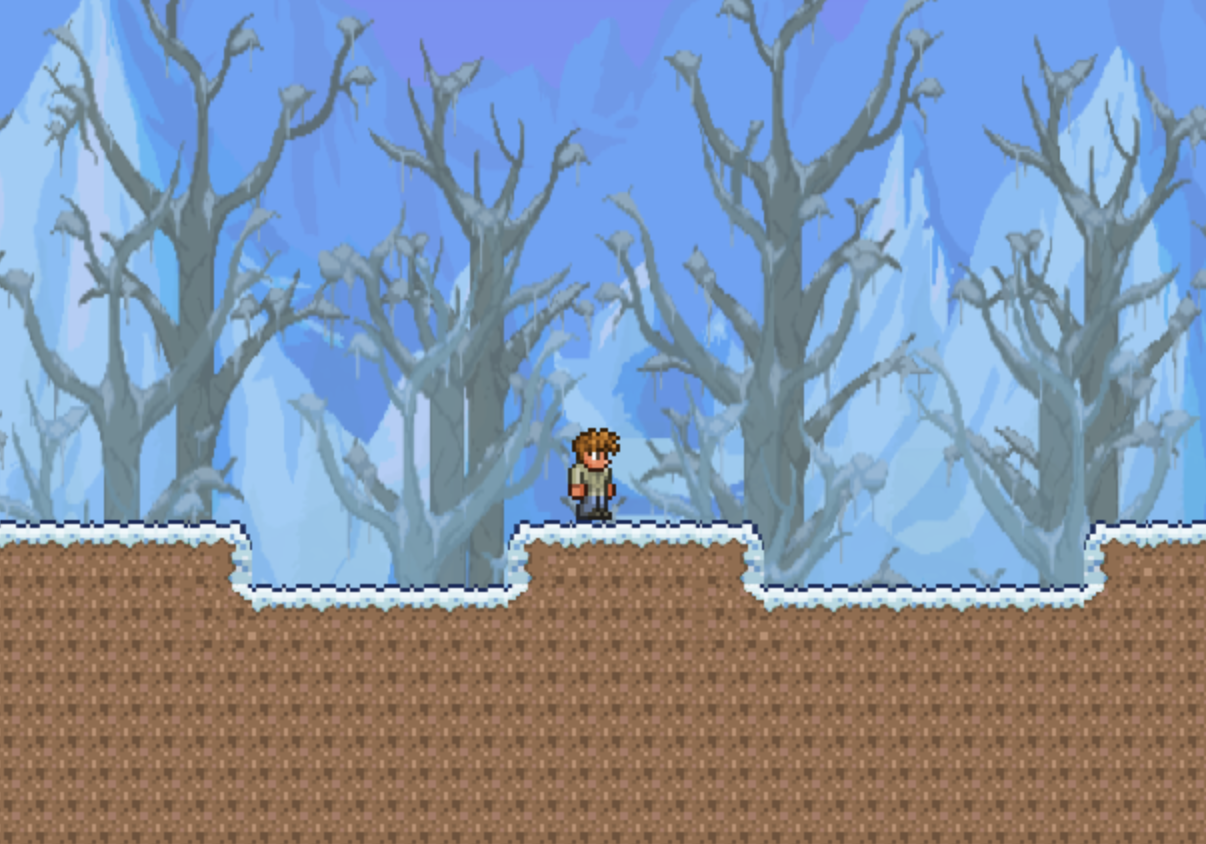
\includegraphics[width=0.5\textwidth]{assets/game_toundra.png}
            \end{figure}
            \begin{figure}
                \centering
                \captionsetup{format=sanslabel}
                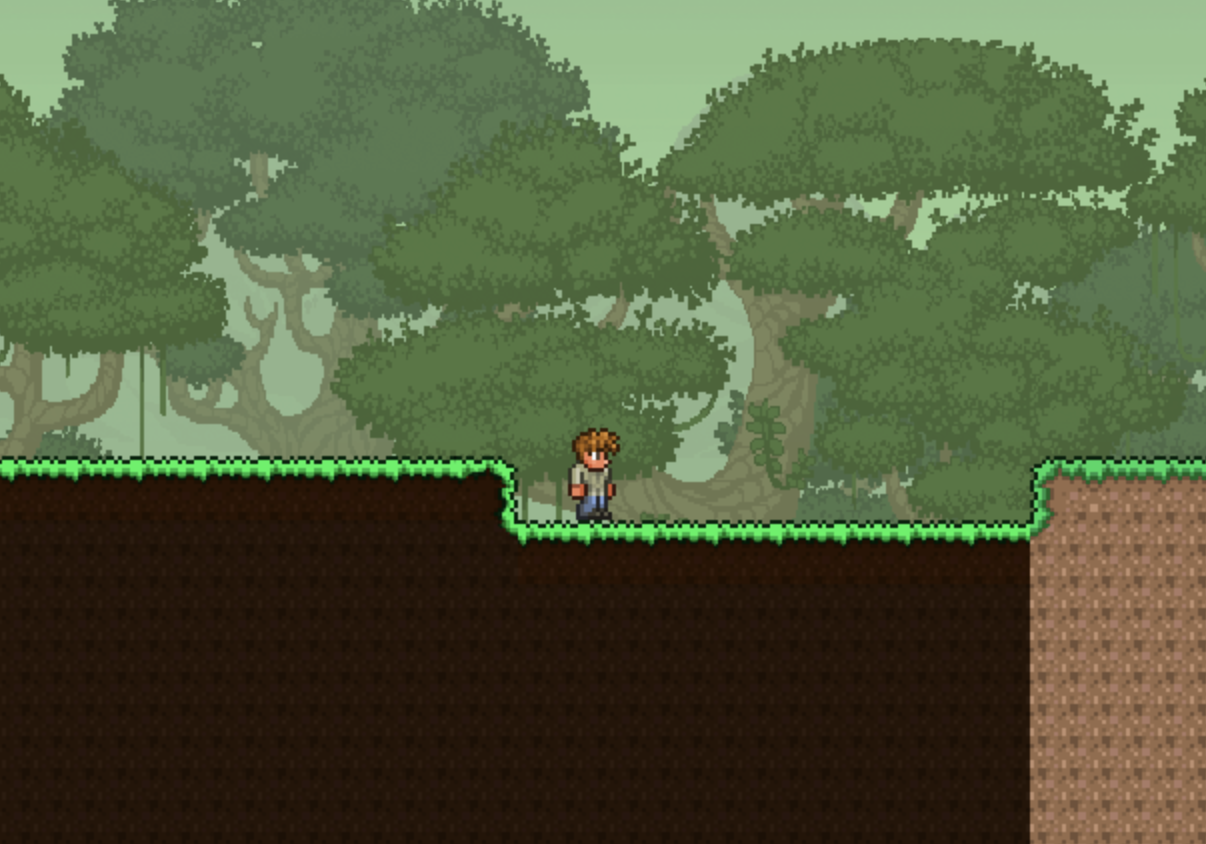
\includegraphics[width=0.5\textwidth]{assets/game_jungle.png}
            \end{figure}
        \end{column}
    \end{columns}
\end{frame}

\subsection{Destruction des blocs}

\begin{frame}{Destruction des blocs}
    \begin{columns}
        \centering
        \begin{column}{0.5\textwidth}
            \centering
            
            \begin{itemize}
                \item \textbf{Fonction} : indicateur visuel, position souris, alignement bloc
                \item \textbf{Comportement} : suivi souris, collision, superposition bloc
                \item \textbf{Destruction bloc} : clic gauche, suppression bloc sélectionné
                \item \textbf{But final (jeu)} : creuser, récolte minerais, fabrication outils/armures
            \end{itemize}
        \end{column}
        \begin{column}{0.5\textwidth}
            \centering
            \begin{figure}
                \centering
                \captionsetup{format=sanslabel}
                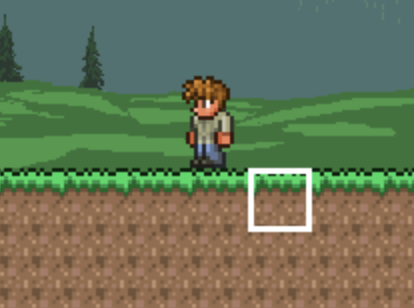
\includegraphics[width=0.5\textwidth]{assets/destruction_1.png}
            \end{figure}
            \begin{figure}
                \centering
                \captionsetup{format=sanslabel}
                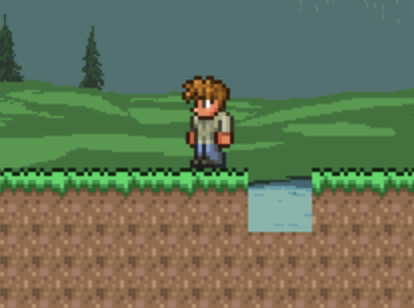
\includegraphics[width=0.5\textwidth]{assets/destruction_2.png}
            \end{figure}
        \end{column}
    \end{columns}
\end{frame}


\section{Résultats}

\begin{frame}{Résultats}
    \begin{columns}
        \centering
        \begin{column}{0.5\textwidth}
            \centering
            \begin{itemize}
                \item \textbf{Type de projet} : jeu immersif, monde ouvert, génération procédurale
                \item \textbf{Déplacement joueur} : exploration libre, terrains variés, seed, unicité
                \item \textbf{Collisions} : détection, interactions cohérentes, physique jeu
                \item \textbf{Caméra} : dynamique, suivi joueur, mode spectateur, exploration aérienne
                \item \textbf{Terrain modifiable} : destruction blocs, creuser, interaction environnement
            \end{itemize}
        \end{column}
        \begin{column}{0.5\textwidth}
            \centering
            \begin{figure}
                \centering
                \captionsetup{format=sanslabel}
                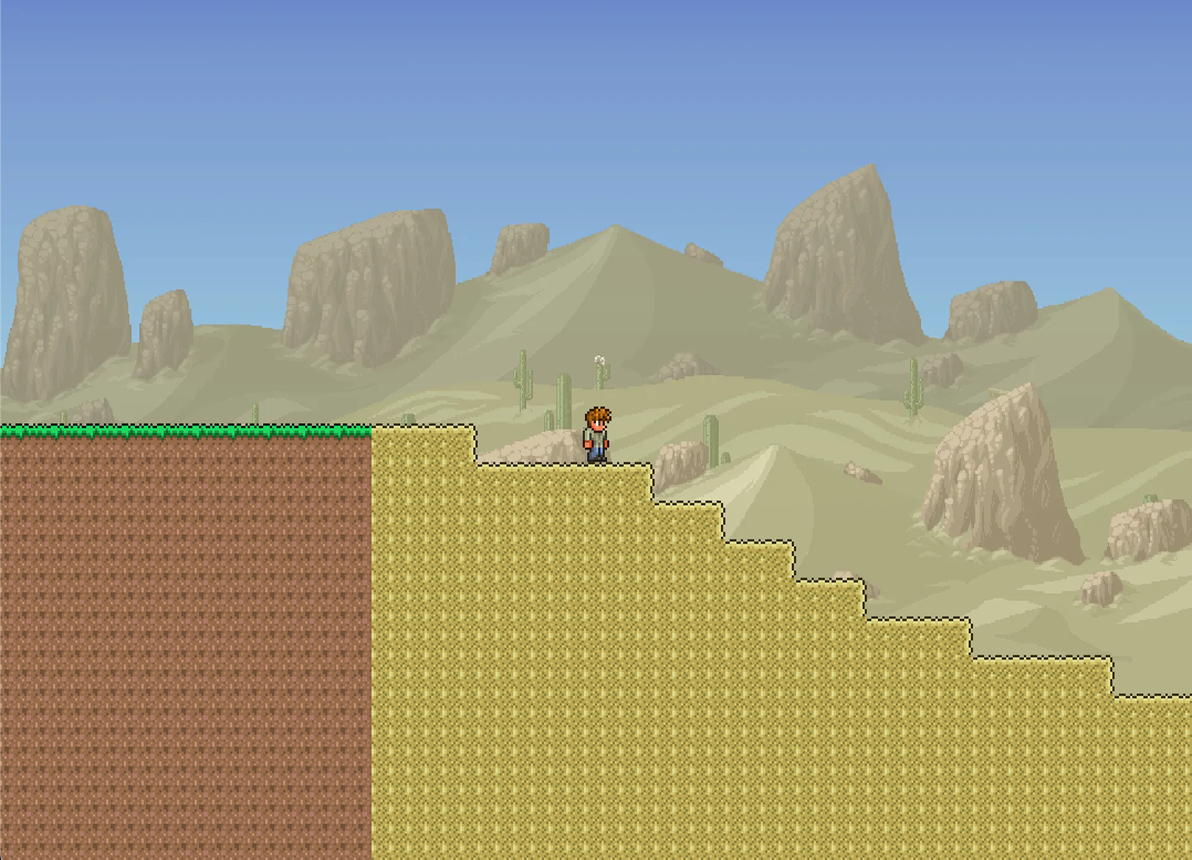
\includegraphics[width=0.9\textwidth]{assets/background_1.png}
            \end{figure}
        \end{column}
    \end{columns}
\end{frame}


\section{Conclusion et Perspectives}

\begin{frame}{Conclusion et Perspectives}
    \centering
    \begin{itemize}
        \item \textbf{Objectif \& choix} : génération procédurale, étude d’algorithmes, inspiration Terraria
        \item \textbf{Résultats} : terrains/biomes générés par seed, mécaniques de base (déplacement, saut, cassage)
        \item \textbf{Limites} : pas de grottes/minerais, pas de montagnes, optimisation à améliorer
        \item \textbf{Apprentissages techniques} : génération procédurale, POO, Python, bonnes pratiques
        \item \textbf{Travail en équipe} : collaboration, outils (Jira, Git), gestion de projet
    \end{itemize}
\end{frame}


\begin{frame}{}
    \centering
    \vfill
    \huge\textbf{Avez-vous des questions ?}
    \vfill
\end{frame}


\end{document}